% -----------------------------------------------------------------------------
% Template from
% https://it.overleaf.com/articles/the-parallelization-and-optimization-of-the-n-body-problem-using-openmp-and-cuda/jpkcgbptkvby
% -----------------------------------------------------------------------------
\documentclass[letterpaper, 10 pt, conference]{ieeeconf}
\IEEEoverridecommandlockouts                              % This command is only
% needed if you want to
% use the \thanks command
\overrideIEEEmargins
% See the \addtolength command later in the file to balance the column lengths
% on the last page of the document


% The following packages can be found on http:\\www.ctan.org
\usepackage{graphics} % for pdf, bitmapped graphics files
\usepackage{epsfig} % for postscript graphics files
%\usepackage{mathptmx} % assumes new font selection scheme installed
%\usepackage{times} % assumes new font selection scheme installed
\usepackage{amsmath} % assumes amsmath package installed
\usepackage{amssymb}  % assumes amsmath package installed

\usepackage{url}
%\usepackage{algorithm}
\usepackage{verbatim}
%\usepackage[noend]{algpseudocode}
\usepackage{soul, color}
\usepackage{lmodern}
\usepackage{fancyhdr}
\usepackage[utf8]{inputenc}
\usepackage{fourier}
\usepackage{array}
\usepackage{makecell}

\renewcommand\theadalign{bc}
\renewcommand\theadfont{\bfseries}
\renewcommand\theadgape{\Gape[4pt]}
\renewcommand\cellgape{\Gape[4pt]}

\newcommand{\rework}[1]{\todo[color=yellow,inline]{#1}}

\makeatletter
\newcommand{\rom}[1]{\romannumeral #1}
\newcommand{\Rom}[1]{\expandafter\@slowromancap\romannumeral #1@}
\makeatother

\pagestyle{plain}

\title{\LARGE \bf
Analysis of the Spatial Covariance Shift in Weather Inference
}
\author{Simone PAPICCHIO, Federico TIBLIAS, Massimo PRONESTI, Daniele FALCETTA% <-this % stops a space 
\\EURECOM - Department of Data Science \\
Sophia Antipolis, France\\
{\tt\small\{name.surname\}@eurecom.fr} \\ \\
}


\begin{document}


    \maketitle
    \thispagestyle{plain}
    \pagestyle{plain}


%%%%%%%%%%%%%%%%%%%%%%%%%%%%%%%%%%%%%%%%%%%%%%%%%%%%%%%%%%%%%%%%%%%%%%%%%%%%%%%%
\section{INTRODUCTION}
    When the distribution of the train and test data differs, this is known as dataset shifting. This may produce several problems because the model is trained on one distribution but it is used to predict different data distributions, resulting in poorer results. There are different types of data shifting such as 
    Covariance Shift\footnote{Changes in the independent variables or features of the dataset},
    Probability Shift\footnote{Changes in the target variable or the dependent variable in the dataset}
    and Concept Shift.\footnote{Change in the connection between the independent and the target variable across datasets}
    In this work we analyze the presence of the Spatial Covariance Shift and try to address its main challenges.

    The data consists of pairs of meteorological features and target values at a particular latitude/longitude and time.
    The Regression task consist in predict the target value which is an air temperature measurements at 2 metres above the ground.
    The features are:
    \begin{itemize}
        \item \textit{weather-related features:} sun evaluation at the current location, climate values of temperature, pressure and topography, and meteorological parameters on different pressures
        \item \textit{surface levels} from weather forecast model predictions.
    \end{itemize} 
    Weather forecast model predictions are values produced by the following weather forecast models: 

    \begin{itemize}
        \item Global Forecast System \textit{(GFS)}
        \item Global Deterministic Forecast System from the Canadian Meteorological Center \textit{(CMC)}
        \item Weather Research and Forecasting \textit{(WRF) }
    \end{itemize}
    Each model returns the following predicted values: wind, humidity, pressure, clouds, precipitation, dew point, snow depth, air and soil temperature characteristics. Where applicable, the predictions are given at different isobaric levels from 50 hPa (20 km above ground) to the ground level.

    Altogether, there are 111 features in total. It is important to note that the features are highly heterogeneous, i.e., they are of different types and scales.

    The main challenge of this dataset is the Spatial Covariance Shift from train to test as is visible in Fig. \ref{fig:train-test-diff}

    \begin{figure}
        \centering
        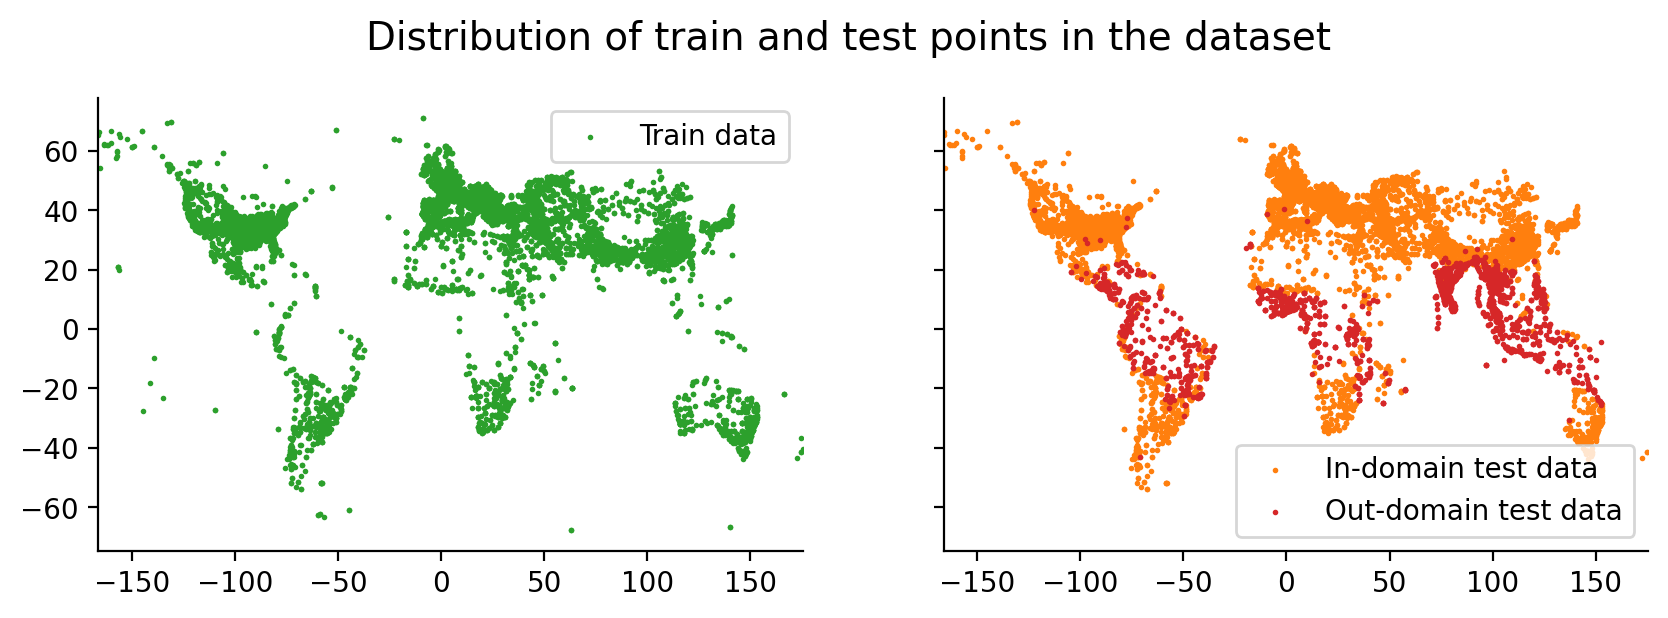
\includegraphics[width=\linewidth]{assets/train-test-diff.png}
        \caption{The figure clearly shows that the regions in the range of latitude from -18 to 10 are not present in the train dataset. This phenomenon is called \textit{Spatial Covariance Shift}. [best visualization in colors] }
        \label{fig:train-test-diff}
    \end{figure}

    \section{Data Analyses}
    
    \subsection{Outliers}
    \subsection{Correlations}
    \subsection{Feature Shift}
    Train and test datasets show a noticeable shift in the distribution of samples: test datapoints are distributed homogeneously around the globe, while train ones are only 
    To gain a deeper understanding of how this phenomenon affects our prediction we compute a metric reminiscent of the Wasserstein distance. For each feature we divide the dataset 100 bins of equal size and normalize them in order to obtain histograms. Then, we compute the cumulative sum of these histograms. Finally we compute the difference between the cumulative area of train and test histograms. The value we obtain represents some notion of distance between the two distributions and can be used later on during feature selection. We report in Table 1 the 10 most shifted features according to this metric. 
    
    \section{Pre-Processing}
    Different models call for different preprocessings. We try different approaches in conjunction with one or more models to find the best one in each situation.
    \begin{itemize}
        \item \textit{Filling missing values with column mean}
        \item \textit{Dropping samples with missing values}
        \item \textit{Feature selection based on Random Forest feature importance:} Train a Random Forest to predict the target value and  keep only the $n$ most important features according to the model. 
        % Fill in the others.
        
    \end{itemize} 
    
    \section{Models}
    
    \section{Hyper-parameter tuning}
    
    \section{result}
    
    \section{conclusion}
%%%%%%%%%%%%%%%%%%%%%%%%%%%%%%%%%%%%%%%%%%%%%%%%%%%%%%%%%%%%%%%%%%%%%%%%%%%%%%%%

\end{document}
